\tasknumber{2018}{16} Вокруг равностороннего треугольника АВС описана окружность радиуса 10. Найдите радиус вписанной
окружности.

\begin{figure}[h]
	\center{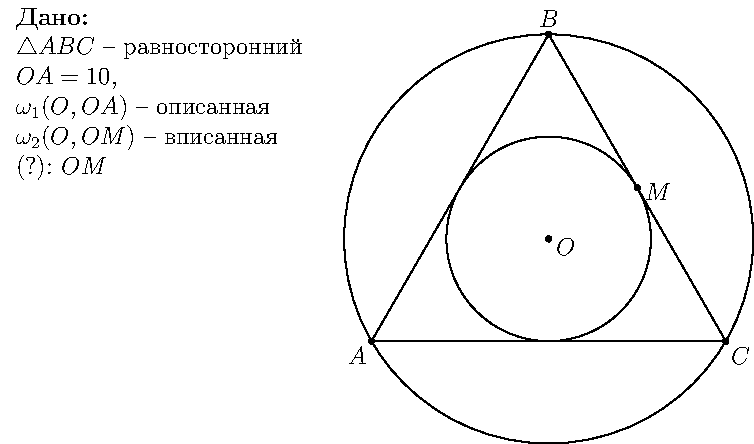
\includegraphics[scale = 1]{task_pic.pdf}}
	%\caption{ }\label{ris:task}
\end{figure}
\Solution
\begin{enumerate}
\item Проведем $BH \perp AC$, $AD \perp BC$, $BD$
\begin{figure}[h]
	\center{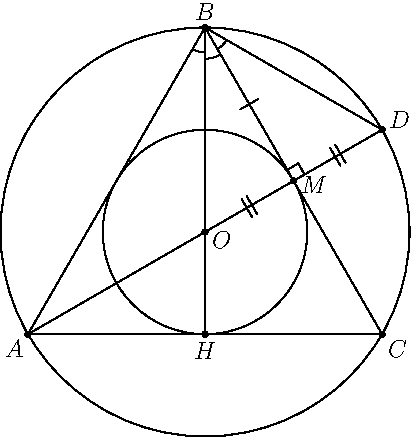
\includegraphics[scale = 0.8]{pic.pdf}}
	%\caption{ }\label{ris:task}
\end{figure}

\item Так как BH -- высота в равностороннем треугольнике, то BH также является биссектрисой.
\item Тогда $\angle ABH = \angle HBC =30^\circ$.
\item Так как $\angle ABD$ опирается на диаметр AD, то $\angle ABD=90^\circ$.
\item Поскольку $\angle ABD=\angle ABH+\angle HBC + \angle CBD = 90^\circ$, получаем равенство: $\angle CBD = 90^\circ -60^\circ=30^\circ $.
\item Откуда $\angle CBD = \angle HBC$ .
\item Тогда $\triangle OBM = \triangle BMD$ по второму признаку ($\angle CBD = \angle HBC$, $\angle OMB = 90^\circ$, $BM$ -- общая сторона).
\item Отсюда получаем, что $OM = \frac{1}{2}OD$
\item Так как OA и OD -- радиусы окружности $\omega_1$, то $OM = \frac{1}{2}OA=5$
\end{enumerate}

\Answer{$OM=5$}
